\chapter{Rewriting math equations into basic UREs}

Based on the work of Gusev and Evans~\cite{broadcastElim,broadcastElimQR},  we can translate math equations into UREs, following the simple steps below. Going through an example, we would find that this process is pretty much mechanical and intuitive, and only middle-school level of math knowledge is needed. So do not be scared by the math symbols. In fact, you want to work out the UREs through the simple math process, since the correctness can be proved and that would save you time in debugging.

We strongly recommend a beginner tries one example so as to quickly master the skills. These skills are generally applicable to real world problems.

Use auto-regressive filter~\cite{autoRegressiveModel} for example:
\begin{equation}
 X_t=c+\sum\limits^I_{i=1}\varphi_i X_{t-i}+\varepsilon_t
\end{equation}
where $c$ is a constant, $\varphi_1, ... \varphi_I$ are the parameters, $\varepsilon _t$ is white noise, and $X_t$ is the output at the current time $t$ and is dependent on the previous $I$ outputs $ X_{t-1}, ..., X_{t-I}$. 

Table~\ref{tab:deriving-ures-for-auto-regressive-filter} shows a complete process how UREs are derived for the problem, and the steps are explained in more detail below:

\begin{table*}[!ht]
\begin{tabular}{|l|ll|ll|}
\hline
    \multicolumn{1}{|c|}{\textbf{Step}} & \multicolumn{2}{|c|}{\textbf{Equations}} & \multicolumn{2}{|c|}{\textbf{Initial values}} \\\hline\hline
     \multirow{1}{*}{1: Iterative form}
        & $X_t=c+\sum\limits^I_{i=1}\varphi_i X_{t-i}+\varepsilon_t$    & $t=1, ..., T$   & $X_{t-i}=0$ &if $t-i \le 0$          \\\hline
     \multirow{2}{*}{2: Recursive form}
        & $X_t=X_t+\varphi_i X_{t-i}$                   & $t=1,...,T$ & $X_t=c+\varepsilon_t$ &  \\
        &                                         &   $i=1,..,I$      &  $X_{t-i}=0$ &if $t-i \le 0$ \\\hline        
     \multirow{2}{*}{3: DSA}
        & $X_t^i=X_t^{i-1}+\varphi_i X_{t-i}^I$         & $t=1,...,T$  & $X_t^{0}=c+\varepsilon_t$ & \\
        &                                         &  $i=1,..,I$& $X_{t-i}^I=0$ &if $t-i \le 0$\\\hline        
     \multirow{2}{*}{4: Full index form}
         & $X_t^i=X_t^{i-1}+\varphi_i^0 X_{t-i}^I$      & $t=1,...,T$ & $X_t^{0}=c+\varepsilon_t^0$  & \\
         & &$i=1,..,I$ & $X_{t-i}^I=0$ &if $t-i \le 0$\\\hline         
     \multirow{4}{*}{5: UREs}
         & \multicolumn{2}{|l|}{$\Phi_t^i=(t-1=0) ? \varphi_i^0 : \Phi_{t-1}^i $}             &    & \\
         & \multicolumn{2}{|l|}{$\chi_t^i=(t-1=0) ? 0 : (i-1=0 ? X_{t-1}^{i-(1-I)} : \chi_{t-1}^{i-1})$}&&\\
         & $X_t^i=(i-1=0 ? c+\varepsilon_t^0 :  X_t^{i-1})+\Phi_t^i\chi_t^i$ &$t=1,...,T$ & &\\
         & & $i=1,..,I$& & \\\hline         
\end{tabular}
\caption{Deriving UREs for auto-regressive filter. Here $c? a : b$ is an expression returning $a$ when condition $c$ is true, and $b$ otherwise.}
\label{tab:deriving-ures-for-auto-regressive-filter}
\end{table*}


\section{Step 1: Iterative form}

First, write down the math equation(s) of the original problem. Usually, in an  equation, a domain  is iterated (like $i=1,...,I$ and $t=1,...,T$),  and some variable (like $X$) is computed. A variable might have some initial values (like $X_{t-i}=0$ for $t-i \le 0$).

\section{Step 2: Recursive form}

Translating the iterative form to a recursive form is straightforward: according to the iterative form, initialize a variable (e.g. $X_t=c+\varepsilon_t$), and update the variable every iteration with a new value based on its previous value (in the form of $X_t=X_t+...$).

\section{Step 3: DSA (Dynamic Single Assignment)}

When updating a variable every iteration, save it to a distinct memory location. Every reference to a variable thus exposes the iteration in which the variable is defined. For example, $X_t=X_t + ... X_{t-i}$ is changed into  $X_t^i=X_t^{i-1} + ... X_{t-i}^I$. After this renaming, it is clear that the 3 references to $X$ are referring to the $X$ values defined in the current iteration $\begin{psmallmatrix}i\\t\end{psmallmatrix}$ and previous iterations $\begin{psmallmatrix}i-1\\t\end{psmallmatrix}$ and $\begin{psmallmatrix}I\\t-i\end{psmallmatrix}$, respectively. 
Consequently, dataflow/dependences between these iterations are made explicit.  

For another example, the initialization $X_t=c+\varepsilon_t$ is changed into  $X_t^0=c+\varepsilon_t$ by adding one 0 for the missing index $i$. $X_t^0$ refers to the $X$ value defined in iteration $\begin{psmallmatrix}0\\t\end{psmallmatrix}$, which is outside the domain, because index $i$ starts from 1 with a step of 1. In general, if index $i$ starts from $s$ with a step $h$, the initial value should be $X_t^{s-h}$.

\section{Step 4: Full index form}

Now variables are referenced with full indices, but constants are not: $\varphi_i$ and $\varepsilon_t$ are inputs never modified when computing $X_t$ (The other constant $c$ is just a number and we do not care). Similar to the handling of initialization in step 3, we give these constants full indices by adding 0's for the missing index $i$:  change $\varphi_i$ and $\varepsilon_t$  into $\varphi_i^0$ and $\varepsilon_t^0$. They refer to the $\varphi$ and $\varepsilon$ values defined in iteration $\begin{psmallmatrix}0\\i\end{psmallmatrix}$ and $\begin{psmallmatrix}0\\t\end{psmallmatrix}$, respectively,  which are outside the domain. In general, if iteration index $i$ starts from $s$ with a step $h$, we should rename $\varphi_i$ and $\varepsilon_t$ into $\varphi_i^{s-h}$ and $\varepsilon_t^{s-h}$.

After being full indexed, variables and constants will be processed in the same way.

At this point, the equations we get are AREs (Affine Recurrence Equations), that is, the current iteration $\begin{psmallmatrix}i\\t\end{psmallmatrix}$ reads a value defined in a previous iteration with a distance $d$ that is in the form of  $d=A\begin{psmallmatrix}i\\t\end{psmallmatrix}+d_0$, where $A$ is a matrix and $d_0$ a constant vector. In other words, there is a read-after-write affine dependence between the two iterations. The dependence distance can be calculated as the current iteration  - the previous iteration  = the write's index - the read's index: Remember that every write/read is fully indexed with the iteration that defines its value; thus the write is indexed with the current iteration, the read is indexed with the previous iteration.  See Table~\ref{tab:deps-full-index-form-auto-regressive-filter} for all the dependences:

\begin{table*}[!ht]
\begin{tabular}{|c|c|c|l|}
\hline
    \multicolumn{1}{|c|}{\textbf{Dependence No.}} & \multicolumn{1}{|c|}{\textbf{Write}} & \multicolumn{1}{|c|}{\textbf{Read}} & \multicolumn{1}{|c|}{\textbf{Dependence distance}}\\\hline\hline
     \multirow{1}{*}{1} & $X_t^i$ & $X_t^{i-1}$ &  $\begin{pmatrix} i\\t\end{pmatrix} -  \begin{pmatrix} i-1 \\ t\end{pmatrix} =  \begin{pmatrix} 1 \\ 0\end{pmatrix}$ \\\hline
     \multirow{1}{*}{2} & $X_t^i$ & $\varphi_i^{0}$ &  $\begin{pmatrix} i\\t\end{pmatrix} -  \begin{pmatrix} 0 \\ i \end{pmatrix} =  \begin{pmatrix} i \\ t-i\end{pmatrix} =  \begin{pmatrix} 1 & 0 \\ -1 & 1\end{pmatrix}  \begin{pmatrix} i \\ t\end{pmatrix}$ \\\hline
     \multirow{1}{*}{3} & $X_t^i$ & $X_{t-i}^{I}$ &  $\begin{pmatrix} i\\t\end{pmatrix} -  \begin{pmatrix} I \\ t-i \end{pmatrix} =  \begin{pmatrix} i-I \\ i\end{pmatrix} =  \begin{pmatrix} 1 & 0 \\ 1 & 0\end{pmatrix}  \begin{pmatrix} i \\ t\end{pmatrix} + \begin{pmatrix} -I \\ 0 \end{pmatrix}$  \\\hline
\end{tabular}
\caption{Dependences of the full index form in  step 4 of  Table~\ref{tab:deriving-ures-for-auto-regressive-filter}}.
\label{tab:deps-full-index-form-auto-regressive-filter}
\end{table*}

\section{Step 5: UREs}

We translate AREs into UREs by converting a broadcast into a pipeline. After that, every dependence has a constant distance uniformly in the entire domain.

There are two ways to convert a broadcast into a pipeline, either graphically or mathematically. 

\subsection{First way to translate AREs into UREs: drawing a dataflow graph}
\label{sec:are-to-ures-with-dfg}

We can draw the dataflow and intuitively figure out how to change a broadcast into a pipeline, as exemplified in Fig.~\ref{fig:broadcast-to-pipeline-arf}. According to the 2nd dependence in Table~\ref{tab:deps-full-index-form-auto-regressive-filter}, originally, a datum $\varphi_i^0$ is broadcast to iterations $X_t^i$ for all $t$, as shown in the left of the figure. 

Equivalently, the same datum can be loaded in an iteration at a boundary of the domain, and from that iteration, propagated in a pipeline fashion to all the other iterations, as shown in the right of the figure. As we can see, $\varphi_i^0$ is  loaded at a bounary iteration $(i, 1)$, and then is propagated to iteration $(i, 2)$, and from there to iteration $(i, 3)$, etc. 

\begin{figure}[!ht]
    \centering
    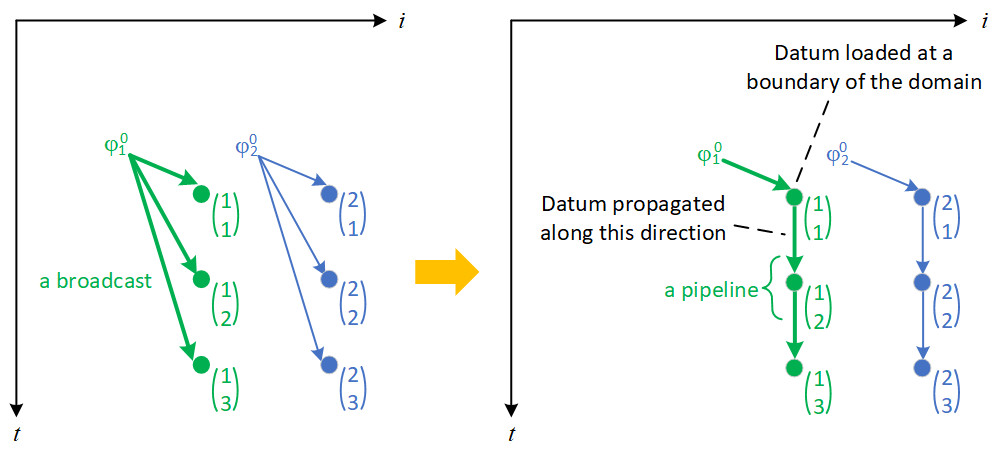
\includegraphics[width=\textwidth]{./img/broadcast-to-pipeline-arf.png}
    \caption{For the 2nd dependence of auto-regressive filter in Tabel~\ref{tab:deps-full-index-form-auto-regressive-filter}, the broadcasts due to this dependence are changed to pipelines. Here we assume $T=3$, and every point is an iteration annotated with its indices $\begin{psmallmatrix} i\\ t\end{psmallmatrix}$.}
    \label{fig:broadcast-to-pipeline-arf}
\end{figure}

\subsubsection{Expressing a pipeline} 
\label{sec:express-pipeline}

Now we can modify the full index form

\begin{equation}
X_t^i=...\varphi_i^0...
\end{equation}

into

\begin{equation}
X_t^i=...\Phi_t^i...
\end{equation}

where $\Phi$ values are propagated along the $t$ dimension until out of the domain:

\begin{equation}
\Phi_t^i=(t-1=0) ? \varphi_i^0 : \Phi_{t-1}^i
\end{equation}

As you can see, the keys to change a broadcast into a pipeline are: (1) the direction of the pipeline, along which data would be propagated from one iteration to the next, and (2) the boundary conditions when the pipeline is fed with some initial values.  

In the same way, we can convert a broadcast due to the third dependence into a pipeline (Could you do it?). After that, we get the UREs shown in step 5 of  Table~\ref{tab:deriving-ures-for-auto-regressive-filter}.

\subsection{Second way to translate AREs into UREs: Calculating a propagation direction}
\label{sec:are-to-ures-with-math}

We can generalize the example in Fig.~\ref{fig:broadcast-to-pipeline-arf}, and directly find out a propagation direction vector in simple math: 

\begin{quotation}
\noindent If a read-after-write dependence is affine, i.e. the distance $d$ is in the form of $Az+d_0$, where $A$ is a matrix, $z$ is the current iteration, and $d_0$ is a constant vector, then the dependence incurs broadcasts of values, and such a broadcast can be changed into a pipeline by propagating a value along a direction $r$ that is a solution of $(E-A)r=\mathbf{0}$, where $E$ is the identity matrix.
\end{quotation}

\begin{figure}[!ht]
    \centering
    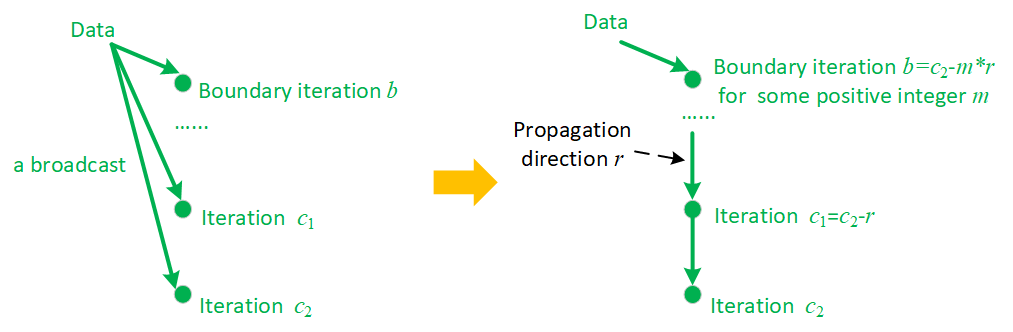
\includegraphics[width=\textwidth]{./img/broadcast-to-pipeline.png}
    \caption{Changing a broadcast into a pipeline}
    \label{fig:broadcast-to-pipeline}
\end{figure}

The left part of Fig.~\ref{fig:broadcast-to-pipeline} shows that due to an affine dependence, some data are broadcast to multiple consumers, including an iteration $b$ at the boundary of the domain, and two other iterations $c_1$ and $c_2$, etc. Remember that data are fully indexed, i.e. they can be considered having been defined in an iteration $y$, even though that iteration is actually out of the domain. 

Let the dependence distance be $d=Az+d_0$.  Because both iteration $c1$ and $c_2$ get data from the same iteration $y$, using the  dependence distance, we have
\begin{equation}
y = c_2 - (Ac_2+d_0) = c_1 - (Ac_1+d_0)
\end{equation}

So
\begin{equation}
(E-A)c_2 = (E-A)c_1    
\end{equation}

Let $r=c_2-c1$, we have
\begin{equation}
(E-A)r = 0.
\end{equation}

Therefore, we can imagine that a datum that is defined outside the domain is first sent to a boundary iteration $b$, and then following a propagation direction $r$ to the next iteration $b+r$, and so on, and eventually the data reach iteration $c_1$, and then $c_2$, etc. This constructs a pipeline as shown in the right part of Fig.~\ref{fig:broadcast-to-pipeline}.

For example, the second dependence for the auto-regressive filter is $\begin{psmallmatrix} 1 & 0 \\ -1 & 1\end{psmallmatrix}  \begin{psmallmatrix} i \\ t\end{psmallmatrix}$ (Table~\ref{tab:deps-full-index-form-auto-regressive-filter}), and thus $A=\begin{psmallmatrix} 1 & 0 \\ -1 & 1\end{psmallmatrix}$. Solve the equation $(E-A)r=\begin{psmallmatrix} 0 & 0 \\ 1 & 0\end{psmallmatrix}r=\mathbf{0}$. We get a solution $r=\begin{psmallmatrix} 0 &\\ *\end{psmallmatrix}$, where the second element (the $t$ dimension)  can be arbitrary. Take a non-zero solution $r=\begin{psmallmatrix} 0 &\\ 1\end{psmallmatrix}$, and we see exactly from the right part of Fig.~\ref{fig:broadcast-to-pipeline-arf} that a  pipeline can be constructed along the $t$ dimension for a datum. 

With this propagation direction, we convert a broadcast due to the second dependence into a pipeline in the same way as shown in Section~\ref{sec:express-pipeline}. Following the same approach, for the third dependence, we can find a propagation direction $r=\begin{psmallmatrix} 1 &\\ 1\end{psmallmatrix}$, and convert the broadcasts due to this dependence into pipelines as well (Could you do it?). After that, we get the UREs shown in step 5 of  Table~\ref{tab:deriving-ures-for-auto-regressive-filter}.

\subsection{Testing correctness of UREs in standard C}
\label{sec:test-correctness-ures}

We can express the UREs in Table~\ref{tab:deriving-ures-for-auto-regressive-filter} in standard C, adding necessary helping code for testing, and see if the UREs can produce correct results. See Listing~\ref{lst:test-correctness-ures-auto-regressive-filter-in-c}.  

\lstinputlisting[language=c, caption={Testing the correctness of the UREs in Table~\ref{tab:deriving-ures-for-auto-regressive-filter} in standard C code.}, label={lst:test-correctness-ures-auto-regressive-filter-in-c}]{code/auto-regressive-filter-testing-ures-in-c.c}


Now test it: 
\begin{verbatim}
    $gcc auto-regressive-filter-testing-ures.c
    $./a.out
    Success!
\end{verbatim}

\subsection{Expressing the UREs in T2S}
\label{sec:express-ures-in-t2s}

It is straightforward to express the UREs in T2S. See Listing~\ref{lst:test-correctness-ures-auto-regressive-filter-in-t2s}. The code is similar to the C code before. The major difference is that the T2S code builds a symbolic dataflow graph where inputs are symbolic parameters and computation is symbolic expressions (Line 13-27), then instantiates the graph to compute with concrete inputs (Line 29-37), and after that compares with a golden baseline for correctness.  

\lstinputlisting[language=c, caption={Testing the correctness of the UREs in Table~\ref{tab:deriving-ures-for-auto-regressive-filter} in T2S.}, label={lst:test-correctness-ures-auto-regressive-filter-in-t2s}]{code/auto-regressive-filter-testing-ures-in-t2s.cpp}

Now test it: 
\begin{verbatim}
    $ export T2S_PATH=path_to_your_t2s_installation
    $ export PATH=$T2S_PATH/Halide/bin:$T2S_PATH/install/gcc-7.5.0/bin:$PATH
    $ export LD_LIBRARY_PATH=$T2S_PATH/Halide/bin:$LD_LIBRARY_PATH
    $ g++ -I$T2S_PATH/Halide/include -L$T2S_PATH/Halide/bin -lHalide  -std=c++11 \   
          auto-regressive-filter-testing-ures-in-t2s.cpp
    $ ./a.out 
    Success!
\end{verbatim}


